%===============================================================
% Utilize este template para construir apresentações da Especialização em Eng. Ferroviária na Faeng-UFMT.
% Atente-se para a estrutura deste arquivo:
%   Linhas 1-281: Configurações do template. Não altere!
%   Linhas 282-299: Definições do autor. Altere apenas seu nome,  
%                   seu curso, nome do orientador, data de
%                   apresentação e título.
%  A partir da linha 300: Corpo da apresentação.
%===============================================================

\documentclass{beamer}
\usefonttheme{serif} % Vous pouvez aussi utiliser {professionalfonts} ou d'autres options

\usepackage[utf8]{inputenc}
%\usepackage{lmodern}
\usepackage{comment}
\usetheme{Madrid}
  \usepackage[maxbibnames=99]{biblatex}
\definecolor{cvut_navy}{HTML}{0065BD}
\definecolor{cvut_blue}{HTML}{6AADE4}
\definecolor{cvut_gray}{HTML}{156570}
\definecolor{faeng_blue}{HTML}{09246F}
\usepackage{biblatex}
%\usepackage{tikz}
%\usepackage{pgfplots}
\usepackage[makeroom]{cancel}
\usepackage{threeparttable}
\usepackage[utf8]{inputenc}
%\usepackage[usenames,dvipsnames]{xcolor}
%\addbibresource{biblatex-examples.bib}
%\setbeamercolor{section in toc}{}
\setbeamercolor{section in toc}{fg=black,bg=yellow} 
\setbeamercolor{alerted text}{fg=cvut_blue}
\usepackage{tikzsymbols}
\usepackage{textcomp}
\usepackage{parskip}
\definecolor{darkblue}{rgb}{0, 0, 0.5} 
\definecolor{babyblue}{rgb}{0.54, 0.81, 0.94}
\usepackage{pgf}
\usepackage[backend=biber]{biblatex}
\addbibresource{ref.bib}

%\usepackage{pythontex} 
\usepackage{tcolorbox}
\tcbuselibrary{skins}
\usepackage{minted}
\usepackage{hyperref}
\usepackage{xcolor,soul}
\definecolor{lightblue}{rgb}{.90,.95,1}
\sethlcolor{lightblue}
\renewcommand<>{\hl}[1]{\only#2{\beameroriginal{\hl}}{#1}}
\setbeamertemplate{page number in head/foot}[totalframenumber]
%%% attravive box over equestion
\usepackage{empheq}
\usepackage{xcolor}
\definecolor{lightgreen}{HTML}{90EE90}
\newcommand{\boxedeq}[2]{\begin{empheq}[box={\fboxsep=6pt\fbox}]{align}\label{#1}#2\end{empheq}}
\newcommand{\coloredeq}[2]{\begin{empheq}[box=\colorbox{lightgreen}]{align}\label{#1}#2\end{empheq}}
\newcommand{\highlight}[1]{%
  \colorbox{red!40}{$\displaystyle#1$}}

  \definecolor{babyblue}{rgb}{0.54, 0.81, 0.94}
\definecolor{babypink}{rgb}{0.96, 0.76, 0.76}
\definecolor{blue(ncs)}{rgb}{0.0, 0.53, 0.74}
\definecolor{pistachio}{rgb}{0.58, 0.77, 0.45}
\definecolor{darksalmon}{rgb}{0.91, 0.59, 0.48}
\definecolor{lightsalmonpink}{rgb}{1.0, 0.6, 0.6}
\definecolor{columbiablue}{rgb}{0.61, 0.87, 1.0}
\definecolor{corn}{rgb}{0.98, 0.93, 0.36}
\definecolor{jonquil}{rgb}{0.98, 0.85, 0.37}
\definecolor{bananayellow}{rgb}{1.0, 0.88, 0.21}
\newcommand{\bert}{\ensuremath{%
  \mathchoice{\includegraphics[height=2ex]{Bert-pic-removebg-preview.png}} 
    {\includegraphics[height=2ex]{Bert-pic-removebg-preview.png}}
    {\includegraphics[height=1.5ex]{Bert-pic-removebg-preview.png}}
    {\includegraphics[height=1ex]{Bert-pic-removebg-preview.png}}
}}
\newcommand{\Tr}{\operatorname{Tr}}
\newcommand{\Arg}{\operatorname{Arg}}
\useoutertheme{infolines}
\newtcbox{\boxedeqn}{
  nobeforeafter,
  colframe=red!70!black,
  colback=red!5,
  boxrule=0.5pt,
  arc=4pt,
  boxsep=5pt,
  left=5pt,
  right=5pt,
  top=5pt,
  bottom=5pt,
}
\usepackage{courier}
%\usepackage{animate}  
\usepackage{expl3}
%\usepackage[listings,theorems]{tcolorbox}

%%%%%%%%%%%%%%%%%%%%%%%%%%%%%%%%%%%%%%%%%%%%%%%%%%%%%%%%%%%%%%%%%%%%%  
%commands for simulating terminal in/output  
%\scroll[<line separator string>]{<width as TeX dim>} 
%                             {<number of lines>}{terminal text line}  
%\clearbuf  %clears line buffer  
%%%%%%%%%%%%%%%%%%%%%%%%%%%%%%%%%%%%%%%%%%%%%%%%%%%%%%%%%%%%%%%%%%%%%  

\newcommand\scroll[4][§§]{
  \seq_set_split:Nnn\g_inputline_seq{#1}{#4}
  \seq_map_inline:Nn\g_inputline_seq{
    \seq_gput_right:Nx\g_linebuffer_seq{##1}
    \int_compare:nT{\seq_count:N\g_linebuffer_seq>#3}{
      \seq_gpop_left:NN\g_linebuffer_seq\dummy
    }
  }
  \fbox{\begin{minipage}[t][#3\baselineskip]{#2}
    \ttfamily
    \seq_map_inline:Nn\g_linebuffer_seq{\mbox{##1}\\}
  \end{minipage}}
}
\newcommand\clearbuf{\seq_gclear:N\g_linebuffer_seq}
\ExplSyntaxOff

\setbeamertemplate{headline}{%
\begin{beamercolorbox}[colsep=1.5pt]{upper separation line head}
\end{beamercolorbox}
\begin{beamercolorbox}{section in head/foot}
    \vskip2pt\insertsectionnavigationhorizontal{\paperwidth}{}{\hskip0pt plus1filll}\vskip2pt
\end{beamercolorbox}%

\begin{beamercolorbox}[colsep=1.5pt]{lower separation line head}
\end{beamercolorbox}
}
\makeatletter
\newcommand\SoulColor{%
  \let\set@color\beamerorig@set@color
  \let\reset@color\beamerorig@reset@color}
\makeatother
\SoulColor
\usepackage{amsmath, bm}
\usepackage{tikz}
\setbeamercovered{dynamic}

\newcommand{\highlightt}[1]{%
  \colorbox{blue!40}{$\displaystyle#1$}}

\newenvironment<>{problock}[1]{%
  \begin{actionenv}#2%
      \def\insertblocktitle{#1}%
      \par%
      \mode<presentation>{%
       % \setbeamercolor{block title}{fg=white,bg=orange!20!black}
        %\setbeamercolor{block title}{fg=white,bg=red!10!black}
        \setbeamercolor{block title}{fg=white,bg=babyblue}
       \setbeamercolor{block body}{fg=black,bg=white!50}
       \setbeamercolor{itemize item}{fg=orange!20!black}
       \setbeamertemplate{itemize item}[triangle]
     }%
      \usebeamertemplate{block begin}
    \par\usebeamertemplate{block end}
    \end{actionenv}
    }
    
    \newcommand<>{\uncovergraphics}[2][{}]{
    % Taken from: <https://tex.stackexchange.com/a/354033/95423>
    \begin{tikzpicture}
    \node[anchor=south west,inner sep=0] (B) at (4,0)
        {\includegraphics[#1]{#2}};
    \alt#3{}{%
        \fill [draw=none, fill=background, fill opacity=0.9] (B.north west) -- (B.north east) -- (B.south east) -- (B.south west) -- (B.north west) -- cycle;
    }
    \end{tikzpicture}
}

\newlength\dlf
\newcommand\alignedbox[3][yellow]{
  % #1 = color (optional, defaults to yellow)
  % #2 = before alignment
  % #3 = after alignment
  &
  \begingroup
  \settowidth\dlf{$\displaystyle #2$}
  \addtolength\dlf{\fboxsep+\fboxrule}
  \hspace{-\dlf}
  \fcolorbox{red}{#1}{$\displaystyle #2 #3$}
  \endgroup
}

\usepackage{collcell}
\usepackage{booktabs}
\usepackage{etoolbox}
%\usepackage{remreset}% tiny package containing just the \@removefromreset command
\makeatletter

\usepackage{xcoffins}
\NewCoffin\tablecoffin
\NewDocumentCommand\Vcentre{m}
  {%
    \SetHorizontalCoffin\tablecoffin{#1}%
    \TypesetCoffin\tablecoffin[l,vc]%
  }
  
\usepackage{pgfpages}

%% Important 
%%% show note or disable note. 
%\setbeameroption{show notes on second screen=right} % Both

\setbeamertemplate{note page}{\pagecolor{gray!5}\insertnote}\usepackage{palatino}
\usepackage{xcolor}
\usepackage{soul}
\usepackage{etoolbox}
\makeatletter
%\patchcmd{\slideentry}{\ifnum#2>0}{\ifnum2>0}{}{\@error{unable to patch}}% replace the subsection number test with a test that always returns true
\makeatother

%\setbeamercolor*{palette primary}{bg=cvut_navy,fg=gray!20!white}
\setbeamercolor*{palette primary}{bg=faeng_blue,fg=gray!20!white}
\setbeamercolor*{palette secondary}{bg=faeng_blue,fg=gray!20!white} % no color
%\setbeamercolor*{palette secondary}{bg=cvut_navy,fg=cvut_navy}
%\setbeamercolor*{palette secondary}{bg=cvut_blue,fg=white}
\setbeamercolor*{palette tertiary}{parent=palette primary} % color of the top and date
\setbeamercolor*{palette quaternary}{fg=faeng_blue,bg=gray!5!white}
\setbeamercolor*{sidebar}{fg=faeng_blue,bg=gray!15!white}
\usepackage[first=0,last=9]{lcg}
\newcommand{\ra}{\rand0.\arabic{rand}}
\usepackage{color, colortbl}
\usepackage{stackengine,tikz}
\usepackage{transparent}
\usepackage{pgfpages}
\usepackage{graphicx}% http://ctan.org/pkg/graphicx
\usepackage{booktabs}% http://ctan.org/pkg/booktabs
\colorlet{Gray}{gray!30}    
\newcommand*{\MinNumber}{0}%
\newcommand*{\MaxNumber}{0.4}%
\definecolor{bubblegum}{rgb}{0.99, 0.76, 0.8}
\newcommand{\ApplyGradient}[1]{%
  \pgfmathsetmacro{\PercentColor}{100.0*(#1-\MinNumber)/(\MaxNumber-\MinNumber)}%
  \edef\x{\noexpand\cellcolor{babyblue!\PercentColor}}\x\textcolor{black}{#1}%
}
\newcolumntype{R}{>{\collectcell\ApplyGradient}{c}<{\endcollectcell}}

% Ajoutez cette ligne pour enlever les sections du bandeau
\setbeamertemplate{headline}{}

\setbeamercolor{titlelike}{parent=palette primary}
\setbeamercolor{frametitle}{parent=palette primary}

\setbeamercolor{B}{bg=red!30,fg=black}

\setbeamertemplate{section in toc}[default]
\setbeamercolor{itemize item}{fg=black}
\setbeamertemplate{itemize item}[triangle]

\setbeamercolor*{separation line}{}
\setbeamercolor*{fine separation line}{}

\setbeamertemplate{navigation symbols}{} 
\setbeamertemplate{caption}{\raggedright\insertcaption\par}

\setbeamercolor*{block title example}{fg=white,bg=purple!75!black}
\setbeamercolor*{block body example}{fg= black, bg= white}

\definecolor{perso}{rgb}{0.54, 0.81, 0.94}}

\setbeamercolor{itemize item}{fg=perso} % all frames will have red bullets
\setbeamercolor{block title}{bg=red!30,fg=black}
\setbeamertemplate{subsection in toc}[subsections numbered]

\usepackage{eqnarray,amsmath}
\usepackage{amsfonts}
\usepackage{amssymb}
\usefonttheme{professionalfonts}
\usepackage{graphicx}
\usepackage{booktabs} 
\usepackage{bm}
\usepackage{mathtools}
\usepackage[utf8]{inputenc}
\usepackage[T1]{fontenc}
\usepackage[french]{babel}
\usepackage{lmodern} 
\usepackage{booktabs}

\setbeamercolor{block title}{fg=black, bg=yellow}
\setbeamercolor{block2}{use=structure,fg=white,bg=purple!75!black}
% definice makra
\def\bq{\mbox{\kern.1ex\protect\raisebox{-1.3ex}[0pt][0pt]{''}\kern-.1ex}}
\def\eq{\mbox{\kern-.1ex``\kern.1ex}}
\def\ifundefined#1{\expandafter\ifx\csname#1\endcsname\relax }%
\ifundefined{uv}%
        \gdef\uv#1{\bq #1\eq}
\fi


\usepackage{algpseudocode}
\usepackage{ragged2e}
\usepackage{csquotes}

\usepackage{memhfixc}

%====================================================
%========== DEFINITION OF AUTHORS ETC...=============
%====================================================

\author[CentraleSupélec]{}
\institute[]{

    \vspace{-31pt} \\ 
    \begin{figure}
        \centering
        
\includegraphics[height = 1cm]{Beamer/cpdp.png}
        \label{fig:enter-label}
    \end{figure}
    \vspace{8pt} \\ 
    \scriptsize
    \textbf{Auteurs :}  \\ 
	Edward LUCYSZYN^1\\
    Nabil ALAMI^1 \\
    Raphaël PAIN DIT HERMIER^1 \\
    Paul SOURISSE^1 \\
    \vspace{4pt}
    \textbf{Encadrante :}  \\ 
    Anna ROZANOVA-PIERRAT^2

    \vspace{4pt}
    $^1$ \textit{CentraleSupélec, deuxième année cursus ingénieur, pôle-projet "formation à la recherche"}\\
    $^2$ \textit{Laboratoire MICS, CentraleSupélec}\\

}

\title[Congrès Junior Pluridisciplinaire]{ Étude Paramétrique d’un Liner Acoustique}

\date[23/05/2024]{\small{23 mai 2024}}

%====================================================
%========== BEGINNING OF DOCUMENT ===================
%====================================================

\begin{document}

\begin{frame}[plain]
	\titlepage
    \vspace{-1cm}
	\begin{center}%
  		
\includegraphics[height=0.63cm]{Beamer/multiple_logos.png}
	\end{center}
\end{frame}

% =========================================

\begin{frame}{Contexte}
    % \begin{figure}
    %     \centering
    %     
\includegraphics[width=0.45\linewidth]{Beamer/Onera-bloc-marque.png}
    
    % \end{figure}
    \begin{center}
        \Large \textbf{Comment diminuer la pollution acoustique dans un réacteur d'avion ?}\\ \\
    \end{center}
    \vspace{10pt}
    \footnotesize
    \begin{itemize}
        \item \underline{Liners acoustiques :} revêtements appliqués sur les parois internes de la nacelle du moteur, et utilisent le principe de résonance de Helmholtz pour dissiper l'énergie acoustique et donc diminuer le bruit.
    \end{itemize}
    \begin{figure}
        \centering
        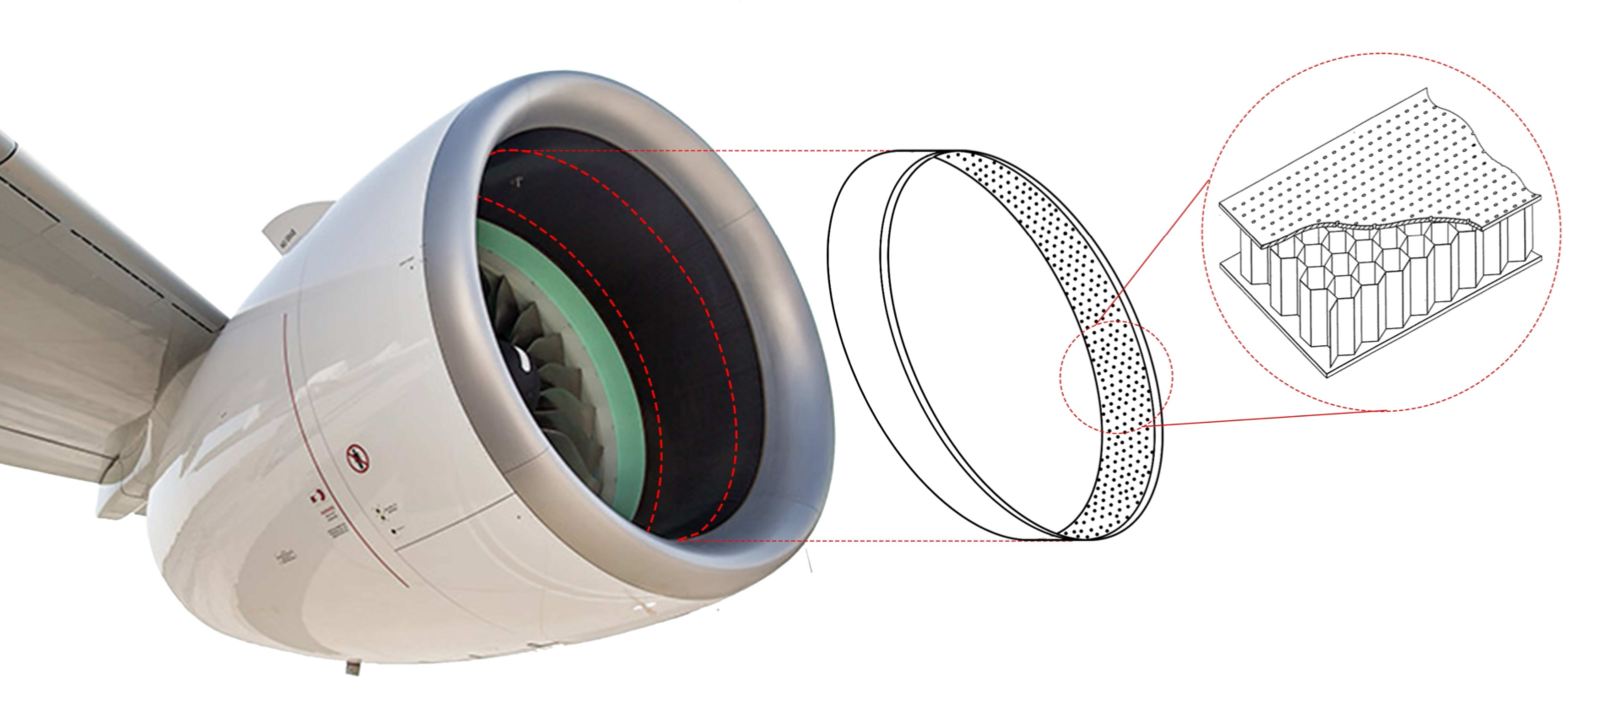
\includegraphics[width = 0.7 \textwidth]{Beamer/liner_photo.png}
        \caption{\footnotesize Liner acoustique appliqué sur la paroi d'un réacteur d'avion. \cite{1}}
        \label{fig:enter-label}
    \end{figure}
\end{frame}



\begin{frame}{Conditions aux bords}
    \begin{center}
    \begin{tikzpicture}
    
        % Côté gauche en noir et plus gros
        \draw[black, ultra thick] (0,0) -- (0,3) node[midway, left] {$\Gamma_{in}$};
        
        % Côté droit en vert
        \draw[black, ultra thick] (6,0) -- (6,3) node[midway, right] {$\Gamma_{out}$};
        
        % Côté en bas en rouge
        \draw[blue, ultra thick] (0,0) -- (6,0) node[midway, below] {$\Gamma$};
        
        % Côté en haut en rouge
        \draw[blue, ultra thick] (0,3) -- (6,3) node[midway, above] {$\Gamma$};
        

        \draw[very thick, ->] (-0.5,-0.5) -- (0.5, -0.5) node[below] 
        {$\vec{\textbf{e}_x}$};

        \draw[very thick, ->] (-0.5,-0.5) -- (-0.5, +0.5) node[left] {$\vec{\textbf{e}_y}$};
        
    \end{tikzpicture}
    \end{center}
    \vspace{-10pt}
    \begin{tcolorbox}
        $$\displaystyle Z\frac{\partial \hat{p}}{\partial n} + i\frac{Z_0}{k_0}\chi Tr ( \mathcal{D}^2\hat{p}) = 0$$
    \end{tcolorbox}
    \footnotesize
    \begin{itemize}
        \item Décrit l'interaction de l'onde acoustique avec la paroi où le liner est posé.
        \item Fondée sur les équations de Navier-Stokes et les travaux de Myers. \cite{2}
    \end{itemize}    
\end{frame}


\begin{frame}{Objectifs du projet}
    \footnotesize
    \begin{itemize}
        \item Cette condition n'est pas réaliste d'après plusieurs expériences. \cite{4}
        \item Les récents travaux de R. Starobinski, Y. Aurégan et V. Pagneux. proposent une approximation plus précise. \cite{6}
        \item $\beta_v \in \mathbb{C}$ est un paramètre complexe dissipatif.
    \end{itemize}

    \begin{tcolorbox}
        \normalsize
        \begin{equation*}
            \frac{\partial p}{\partial n} =\frac{\Upsilon}{i\omega }\bigg(i\omega +(1-\textcolor{blue}{\beta_v})u_0\frac{\partial}{\partial x}\bigg)\bigg(i\omega +u_0\frac{\partial}{\partial x}\bigg)p
        \label{eq3}
        \end{equation*}
    \end{tcolorbox}
    
    \begin{center}
        \large \textbf{\textcolor{perso}{Objectif : }} montrer que le problème est bien posé.
    \end{center}

    
\end{frame}








\begin{frame}{Résultat}

\footnotesize Notre problème s'écrit sous la forme suivante :
\[
    (P_H) \hspace{2pt} : \hspace{2pt}
    \begin{cases}
    \displaystyle \Delta  \hat{p}  + \mathcal{D}^2 \hat{p} = \Tilde{f} \in L^2(\Omega)
    \\
    \displaystyle \displaystyle Z\frac{\partial \hat{p}}{\partial n} + i\frac{Z_0}{k_0}\chi \Tr \Bigl[ \mathcal{D}(\mathcal{D} + iM_0\beta_v\partial_x) \hat{p} \Bigr] = 0\text{ sur }\Gamma \hspace*{2cm} 
    \\
    \displaystyle \Tr(\hat{p}) = 0 \text{ sur } \Gamma_{in}
    \\
    \displaystyle \frac{\partial \hat{p}}{\partial n} + ik \Tr(\hat{p}) = 0 $ sur $\Gamma_{out}
    \end{cases} .
\]
    
\begin{tcolorbox}[colback=cyan!5!white,colframe=perso,title=Notre théorème]
\footnotesize
Soit $\beta_v\in \mathbb{C}$ tel que $|\beta_v| < 1$. Si $\beta_v$ vérifie :

\[\Re e(\frac{1}{Z})\Re e(\frac{\beta_v^2}{1-\beta_v}) - \Im m(\frac{1}{Z})\Im m(\frac{\beta_v^2}{1-\beta_v}) < 0,\]
alors \textbf{le problème $(P_H)$ ci-dessus admet une unique solution faible.} 

\end{tcolorbox}
\end{frame}

\begin{frame}{Valeurs possibles pour $\beta_v$}

\begin{figure}[htbp]
    \centering
    \begin{minipage}[b]{0.45\textwidth}
        \centering
        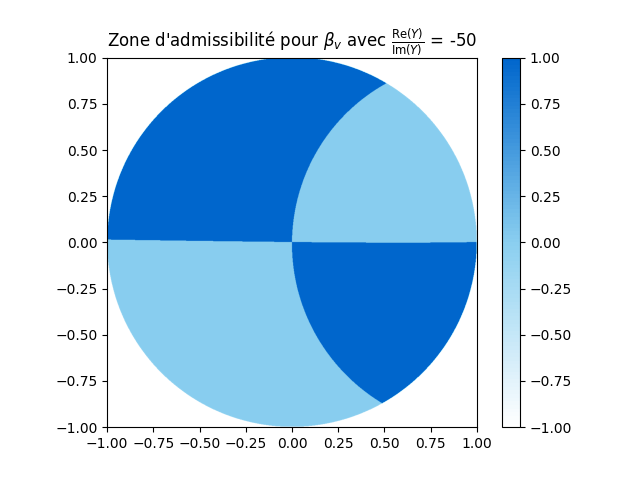
\includegraphics[width=\textwidth]{Beamer/-50.png}
    \end{minipage}
    \hfill
    \begin{minipage}[b]{0.45\textwidth}
        \centering
        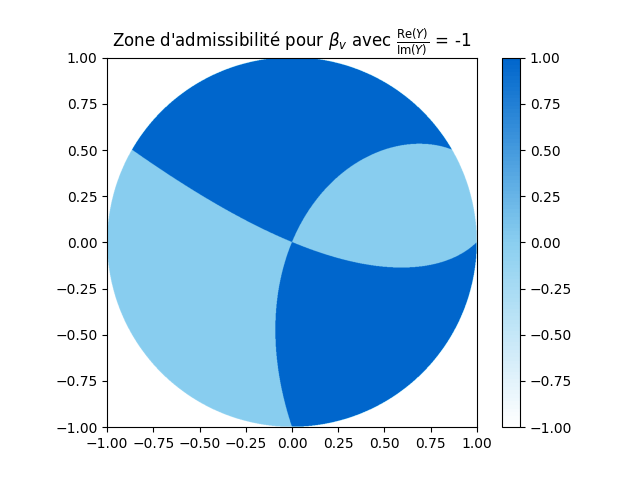
\includegraphics[width=\textwidth]{Beamer/-1.png}
    \end{minipage}
    \vspace{-10pt}
    
    \begin{minipage}[b]{0.45\textwidth}
        \centering
        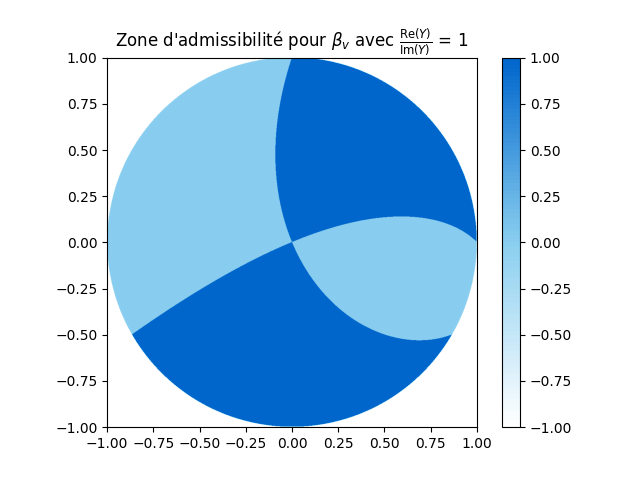
\includegraphics[width=\textwidth]{Beamer/1.png}
    \end{minipage}
    \hfill
    \begin{minipage}[b]{0.45\textwidth}
        \centering
        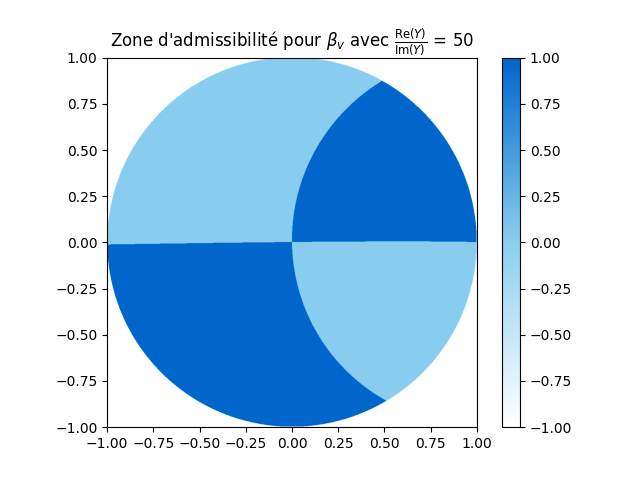
\includegraphics[width=\textwidth]{Beamer/50.png}
    \end{minipage}

    \caption{Figures organisées en 2x2}
    \label{fig:2x2}
\end{figure}
\end{frame}

\begin{frame}{Forme optimale}

Pour $\beta_v$ dans la zone d'admissibilité, nous avons le résultat suivant.

\begin{tcolorbox}[colback=cyan!5!white,colframe=perso,title=Théorème]
Pour \textbf{une quantité} de liners acoustiques \textbf{fixée}, \textbf{il existe une distribution optimale} qui minimise l'énergie du système, et donc \textbf{qui minimise le niveau sonore} pour des données et paramètres fixés.
\end{tcolorbox}
    

\end{frame}


\begin{frame}{}
    \begin{center}
        \Huge \textcolor{faeng_blu}{Conclusion}
        \vspace{20pt}
        \normalsize
        \begin{itemize}
            \item 1) Modèle fréquentiel avec condition de Myers modifié.
            \item 2) Unicité de la solution.
            \item 3) Valeurs de $\beta_v$ et distribution optimale.
        \end{itemize}
    \end{center}
\end{frame}

\begin{frame}{Bibliographie}
    \printbibliography[Bibliographie]
\end{frame}

\end{document}
